\documentclass[11pt]{article}
\usepackage{amsmath}
\usepackage{fullpage}
\usepackage{palatino}
\usepackage{hyperref}
\usepackage{tikz}
\usetikzlibrary{positioning}
\usepackage{natbib, setspace}
\usetikzlibrary{arrows,automata}
\usepackage[latin1]{inputenc}
\usepackage{graphicx}
\usepackage{graphics}

\pagestyle{empty}

\newcommand{\bs}{\boldsymbol}
\newcommand{\mb}{\mathbf}

\begin{document}
\doublespacing

\noindent Computer Science 51: Final Project \hfill \today\\
\noindent\makebox[\linewidth]{\rule{6.5in}{2.0pt}}

\begin{center}

\smallskip
{{\LARGE \bf Blokus Solver}}
\smallskip

\noindent\makebox[\linewidth]{\rule{6.5in}{2.0pt}}

\bigskip

{\large Michelle Cone $|$ Theresa Gebert $|$ Yuan Jiang \\
\normalsize mcone@college.harvard.edu $|$ tgebert@college.harvard.edu $|$ yuanjiang@college.harvard.edu} \\

\end{center}

\bigskip


\begin{center} {\bf Find a link to our demo video \href{http://youtu.be/XVqFYVdfPtk}{here}!} \end{center}


\section{Overview}

Blokus is a popular two- or four-player board game that was invented in 2000. Now there is even an \href{http://forum.blokus.refreshed.be/}{online forum} for avid Blokus players that hosts events and competitions. Blokus is a relatively simple game: it consists of 21 colored Tetris-shaped pieces that players are only allowed to place on a square board cornering their own pieces and non-overlapping any other pieces. Once no more players can place any more pieces, the winner is determined by the player who has the fewest number of points (where one square of a piece is one point).
\\\\
In this project, we set out to write a solver for this game. The implementation of this project can roughly be divided into two parts: constructing the interface of the game, and writing three different solvers. We chose to use object-oriented programming in order to construct the game. The three solvers were chose to implement were:
\begin{enumerate}
	\item {\bf Random} {\it (choose a random piece)}
	\item {\bf Greedy} {\it (choose the ``best" piece, according to a certain score function)}
	\item {\bf Minimax} {\it (choose the ``best" piece by looking ahead one move)}
\end{enumerate}
This report is a discussion of our implementation (including some of its advantages and disadvantages), our results, and a reflection on the success of our project.


\pagebreak


\section{Planning}

Overall, our team was very successful in planning meetings and staying on top of our schedule. We often got goals accomplished ahead of time, though we did end up deviating from our original plan to split up different parts of the project.

\subsection{Timeline}

Our team followed our timeline in the \href{run:report/Functionality_Checkpoint Ann..pdf}{Functionality Checkpoint} and \href{run:report/Final Project Specification (Final) Ann..pdf}{Project Specification Final} very closely by working on our project for a minimum of three to four hours every night. By keeping track of our progress and staying on schedule, we were able to accomplish all of our goals and even implemented two of our three cool extensions.
\\\\
What was particularly effective in our timeline were the daily goals we set for ourselves. In particular, we found our objective to finish a function every night particularly useful. Even if it was just a small helper function, something was added to our project every single day.

%\href{run:report/Functionality_Checkpoint.pdf}{Functionality Checkpoint}
%\href{run:report/Final Project Specification (Draft).pdf}{Project Specification Draft}
%\href{run:report/Final Project Specification (Final).pdf}{Project Specification Final}
% \href{run:report/Random_Players.avi}{Link to video.}

\subsection{Meetings}

Meetings were always scheduled at the end of every meeting. Team members usually showed up on time and time was used efficiently. We also made sure to write down all of our thoughts for functions and classes before implementing them. Particularly when the whole team was together, this brainstorming greatly decreased the amount of code we had to rewrite, because we planned out our code very well. By planning out all of our code first, we were able to make a lot of progress when it  came to actual implementation, even if we were working on parts alone.
\\\\
In addition, the next meeting was often scheduled at the end of every meeting. If it wasn't, we would always be sure to schedule the next one over e-mail within a few hours of the last meeting. This left no ambiguity as to where our project was heading, since all team members always knew when we would see each other next and what had to be accomplished by then.

\subsection{Modularization}

In our original \href{run:report/Final Project Specification (Draft) Ann..pdf}{Project Specification Draft}, we said that we were going to take advantage of our three-person team to implement the three algorithms separately. This did not end up occurring because $1.)$ there was an extreme imbalance in the difficulty of the algorithms (Random was far easier) and $2.)$ the more difficult algorithms, Greedy and Minimax, required more than one person - if not the whole team - to reason through them and code them correctly and efficiently. Therefore, we modified our original plan and ended up working on most of the algorithms together. Debugging was sometimes done alone.


\pagebreak


\section{Implementation}

Recall that our project consisted of two relatively distinct parts: implementing a Blokus game, and implementing the algorithms to solve it. We wrote our code in an iPython Notebook because it was easier to read and comment. It can be found \href{http://nbviewer.ipython.org/github/yuanjiang/blokus_solver/blob/master/Final\%20Project/code/Blokus\%20Solver.ipynb}{here}.

\subsection{The Game}

Implementing a Blokus Solver is challenging because we first had to implement an interface. This was the foundation of our project, since creating a clunky or inefficient interface could make our algorithms very difficult to code. The basic idea is that the Blokus game consists of pieces, players, rules, and a board. Thinking of the rules as methods of a Game object and the pieces, players, and the board as objects with associated methods allowed us to navigate the complex relationships these objects have with each other.

\bigskip

        \definecolor {processblue}{cmyk}{0.96,0,0,0}
        \begin {center}
            \begin {tikzpicture}[-latex ,auto ,node distance =4 cm and 4cm ,on grid, semithick, state/.style ={ circle ,top color =white , bottom color = processblue!20, draw, processblue, text=blue, minimum width =2 cm}]

            %GRAPH
                %initialize nodes
                \node[state] (P) {$Player$};
                \node[state] (Gr) {$Greedy$};
                \node[state] (S) {$Shape$};
                \node[state] (V5) {$V5$};
                \node[state] (Ga) {$Game$};
                \node[state] (B) {$Greedy$};

                %position nodes
	      \node[state] (P) [above =of Gr] {$Player$};
                \node[state] (S) [right=of P] {$Shape$};
	     \node[state] (V5) [below =of S] {$V5$};
                \node[state] (Ga) [right=of S] {$Game$};
	     \node[state] (B) [below =of Ga] {$Blokus$};

                %create + label edges
                \path (Gr) edge node {$inherits$} (P);
                \path (V5) edge node {$inherits$} (S);
                \path (B) edge node {$inherits$} (Ga);

            \end{tikzpicture}
        \end{center}

\bigskip

\noindent A $V5$ is a type of shape (among 20 others) that inherits from the class Shape. Shapes can be rotated and flipped; they also have corners and the points that they occupy on the board. Players have corners that they keep track of, which represent the corners available to them for placement on the board. Players also have pieces, which are removed by the Game when they are played. A Greedy player inherits from a Player but requires additional weights (to be discussed later). We also implement a general Game class which Blokus inherits from to define its own rules. Notice that these relationships can broadly be represented in the following diagram.

\bigskip

\begin{center}
	\begin{tikzpicture}[
	  ->,
	  >=stealth',
	  shorten >=1pt,
	  on grid,
	  node distance=5cm and 3cm,
	  semithick,
	  every state/.style={circle ,top color =white , bottom color = processblue!20, draw, processblue, text=blue, minimum width =1 cm},
	]
	  \node[state]         (P)                     {$Players$};
	  \node[state]         (G) [above right of=P]  {$Game$};
	  \node[state]         (B) [below right of=G]  {$Board$};
	
	  \path[every node/.style={sloped,anchor=south,auto=false}]
	        (G) edge              node {placement} (B)            
	        (G) edge [bend right =35]       node {update} (P)
	        (P) edge [bend right =35]	    node[below] {proposals} (G);
	\end{tikzpicture}
\end{center}

\bigskip

\noindent Rather than permitting the Player to have direct access to the Board, we chose the Game - the rule master, so to speak - to be in charge of asserting that moves proposed by the Player are valid and placing valid moves on the Board. Though this class implementation had a high initial cost in time and code, it made later function calls much shorter and our algorithms more interpretable. For example, one of the highlights of this implementation is the fact that a round can be played with the simple command \texttt{game.play()}.

\subsection{The Algorithms}

Once we had completed the interface and could play the game with naive strategies, we began implementing our algorithms. Recall that our three strategies are Random, Greedy, and Minimax.
\\\\
{\bf Random.} The Random algorithm randomly chooses a Shape object and then randomly chooses among its possible placements. If no placements are available it chooses a different Shape randomly. If no placement is possible it returns \texttt{None}. The resulting board of two Random players playing against each other is expected to look more scattered than the Blokus board of more experienced Blokus players (or our later algorithms).
\\\\
{\bf Greedy.} The Greedy algorithm is based on a score function which weights. A score function - which we name \texttt{eval\_move} - evaluates how ``good" a move is given a particular player and a game. We know, based on the objectives of the game, that larger pieces are better, so our score function takes into account the size of the placement. In addition, we know that corners are important, since we want to minimize the number of future moves for our opponents, but maximize our own. Thus, our score function also takes into the difference between our opponents' corners and our own.
\\\\
However, we would like to generalize this score function such that the difference in corners and the size of the placement are not weighted equally. After all, perhaps it's more important to place large pieces - or perhaps it's more important to gain new corners? In order to make this possible, we define our score function in terms of weights as follows:
\\\\
\indent {\it For a particular placement $i$, we assign weights $W_0$, $W_1$ such that}:

\begin{itemize}
\item $ size_i $ = size ($S$) of placement
\item $ cor_{my} $ = number of my corners ($C$)
\item $ cor_{opp} $ = number of opponent's corners
\item $ n_{opp} $ = number of opponents
\end{itemize}

{\it Then,} $ GreedyEval_i = $

\begin{center} $ size_i W_0 + \left ( \dfrac{\sum{(cor_{my} - cor_{opp})}}{n_{opp}} \right ) W_1 $ \end{center}

\bigskip

\noindent Notice that when $\ n_{opp} = 1 \ $ (as is the case in the two-player game), the evaluation reduces to:
$$ GreedyEval_i = size_i W_0 + (cor_{my} - cor_{opp}) W_1 $$
\noindent Since our original Player class is only defined by a strategy, if we would like to create Players that play according to this Greedy algorithm with particular weights, then we need to be able to pass in weights when we instantiate a Player. This is why we decided to create a Greedy class that inherits from Player.
\\\\
{\bf Minimax.} A Minimax player is essentially just an extension of a a Greedy player that does not only evaluate the current move but looks ahead at future moves. A true Minimax player would look at all possibilities until the end of the game in order to determine his/her next move, but this is computationally infeasible. Therefore, we have chosen to look ahead only one move ahead of the current move. We now need additional weights to determine how many of the possible moves of the first term will be used to look ahead, and how much we want to weight the score of the first move vs. the score of the second move:
\\\\
\indent {\it For a particular placement $i$, we assign weights $W_0$, $W_1$, $W_2$, $W_3$, $W_4$ such that:}

\begin{itemize}
\item $ size_{j,i} $ = size of $j$th placement
\item $ cor_{j,my} $ = number of my corners at $j$th placement
\item $ cor_{j,opp} $ = number of opponent's corners at $j$th placement
\item $ n_{opp} $ = number of opponents
\item $ W_2 $ = number of best placements from initial move that are chosen to run Minimax
\end{itemize}

{\it Then,} $MinimaxEval_{W_2, i} =$

\begin{center} $W_4 \left [ size_{1,i} W_1 + \dfrac{\sum{(cor_{1,my} - cor_{1,opp})}}{n_{opp}} W_2 \right ]
+ W_3 \left [ size_{2,i} W_1 + \dfrac{\sum{(cor_{2,my} - cor_{2,opp})}}{n_{opp}} W_2 \right ]$ \end{center}

\bigskip

\noindent Intuitively, we can see that if we set $W_3$ to $0$, Minimax will be identical to Greedy since we are effectively ignoring the score of the second piece and only maximizing over the score of the first.
\\\\
{\bf User.} The last strategy we implemented was not truly an algorithm, but was a key component of our project. We allowed the user to interact with our algorithms! We had to make several design choices here. We could either have users specify a shape, reference point, orientation, and flip in order to place a shape. But this is very tedious for the user when the game is played on a screen and the user does not have physical pieces to rotate and flip in his/her hands! Another option was to have the user specify a shape and have the game display a list of possible moves. But this is also tedious because the user would need to look through a list of tuples to choose his/her move.
\\\\
We chose to meet somewhere in the middle. Users now specify a reference point and a shape. Users know where reference points are on the pieces according to a pieces map that is displayed at the beginning of the game:

\begin{figure}[h]
\begin{center}
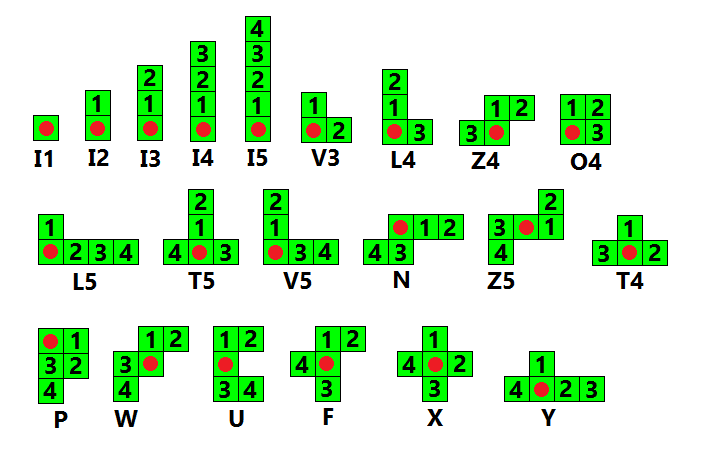
\includegraphics[scale = 0.65]{Blokus_Tiles.png}
\end{center}
\end{figure}

\noindent Given this information, the game is able to generate a (much shorter!) list of possible moves that the user can choose from.


\pagebreak


\section{Analysis}

Developing multiple algorithms gave us the opportunity to play them against each other. This section explores the performance of our algorithms, their advantages and disadvantages, as well as some of the lessons we learned about the game of Blokus in general.

\subsection{Performance}

The following table summarizes the scores of some of our algorithms playing against each other. Recall that $S$:$C$ refers to the ratio between the score weighting and the corners weighting in the Greedy and Minimax algorithms; $Ft$:$Sc$ refers to the ratio between the ratings of the first and second move that are scored in the Minimax algorithm. (Videos pop up by clicking on the scores.)

\bigskip
\begin{center}
\begin{tabular}{|l|l|l|l||r|r|r|}
\hline
{\it Player 1} & {\it Weights 1 } & {\it Player 2} & {\it Weights 2} & {\it Duration} & {\it Score} & {\it Winner} \\
\hline
Random & n/a & Random & n/a & 1:40 & \href{run:report/Videos/Random_v_Random.avi}{rand.} & rand. \\
\hline
Greedy & {\it S:C} = 2:1 & Random & n/a & 2:15 & \href{run:report/Videos/Greedy21_v_Random.avi}{76, 46} & 1 \\
\hline
Greedy & {\it S:C} = 1:2 & Greedy & {\it S:C} = 2:1 & 2:15 & \href{run:report/Videos/Greedy12_v_Greedy21.avi}{67, 74} & 2 \\
\hline
Minimax & {\it S:C} = 2:1, {\it Ft:Sc} = 1:1 & Greedy & {\it S:C} = 2:1 & 4:15 & \href{run:report/Videos/Minimax21511_v_Greedy21.avi}{73, 66} & 1 \\
\hline
Greedy & {\it S:C} = 2:1 & Minimax & {\it S:C} = 2:1, {\it Ft:Sc} = 1:1& 4:15 & \href{run:report/Videos/Greedy21_v_Minimax21511.avi}{71, 72} & 2 \\
\hline
Greedy & {\it S:C} = 1:2 & Minimax & {\it S:C} = 2:1, {\it Ft:Sc} = 1:1 & 4:15 & 63, 77 & 2 \\
\hline
Minimax & {\it S:C} = 1:2, {\it Ft:Sc} = 1:1 & Minimax & {\it S:C} = 2:1, {\it Ft:Sc} = 1:1 & 4:15 & \href{run:report/Videos/Minimax12511_v_Minimax21511}{76, 68} & 2 \\
\hline
\end{tabular}
\end{center}
\bigskip

\noindent Besides the games involving a Random player, the other results are entirely deterministic, since these algorithms will always play identically against each other. We did not incorporate randomness into their piece choices, so their scores will always be the same.
\\\\
An additional parameter for Minimax is not only the weights for the piece size ($S$) vs. players' corner difference ($C$) and the first move ({\it Ft}) vs. second move ({\it Sc}), but also the number of possible moves we would like to look ahead with. Since it would take a much longer time to look ahead an additional move with all possible moves, we allow this number to be bounded by an input parameter. We did not include this in our table of results because we noticed that when we increase this number, it does not change the final score or the final board. From this we gather that it is unlikely a poor first move will result in a second move that could compensate for the first. In short, play a good move the first time around, since it's unlikely you will be able to make up for that mistake on the next move!
\\\\
In addition, notice that the Greedy player that favors size beats the Greedy player that favors corners {\it even though she goes second.} We have noticed repeatedly that there is about a three-point advantage to going first when identical algorithms are playing against each other. So the fact that the size-favoring algorithm wins despite the handicap of going second tells us that the size-favoring Greedy algorithm is truly much better.

\subsection{Lessons}

Running our three algorithms taught us about some important properties of the game of Blokus.

\begin{enumerate}
	\item Running different weightings taught us that the size of a piece is more important than the number of corners you could gain (or your opponent could lose) for any given placement.
	\item We also learned that it is more advantageous for Minimax to play a larger piece on the current turn, even if the combined score of the current and subsequent move is not the maximum over all possible moves. This is because when Minimax has such a shallow depth and can only look a single move ahead, it will not realize that certain moves can prevent the placement of a crucial five-piece later in the game.
	\item When we are playing Minimax and Greedy against each other with the same weighting, then we notice whichever one goes first, wins. We see it's a very clear advantage to go first. Do notice that Minimax wins by more when it goes first.
\end{enumerate}
In addition, watching our best algorithms, like the size-favoring Greedy player, shows us that our algorithms play similar to experienced Blokus players: they move towards the middle as quickly as possible and generally play their larger pieces first.


\pagebreak


\section{Reflection}

Overall, our entire group agrees that, though the project required a lot of work, our planning made it run smoothly and kept us ahead of schedule most of the time. We consider this one of the most successful group projects we have completed to date.

\subsection{Learning}

One of the most important things we learned from the project was learning to code more efficient algorithms. Given that parts of our algorithms can be computationally intensive, we really had to consider all of our options when it came to optimizing code and making our program more efficient. To this end, we made sure to avoid any unnecessary computations (e.g. only sorting when necessary), and inputting subsets of pieces rather than all the pieces to check. In terms of style, we tried to use list comprehensions whenever possible to avoid \texttt{for}-loops, and we made sure to comment our code so that going back to what we did a previous night was easy and clear.

\subsection{Teamwork \& Communication}

Each group member contributed to the project equally. Recall that we initially planned to split up the three algorithms equally and have each person implement one separately. However, we ended up meeting up to implement the classes and algorithms together. Write-ups and final specifications were also divided equally between all members.
\\\\
Communication was what our team excelled in. We communicated our ideas well during meetings and listened to each other's ideas. We also stayed in touch over e-mail, so that when we split up to do separate work everyone still knew what was going on.

\subsection{Time Management}

By working on our project very consistently, we were able to keep on track as dictated by our timeline in the \href{run:report/Final Project Specification (Final) Ann..pdf}{Project Specification Final} and later in the \href{run:report/Functionality_Checkpoint Ann..pdf}{Functionality Checkpoint} as well. We were able to implement two of the cool extensions that we had proposed in the initial project specification. Not only did we include a factor in the evaluation function that took into consideration how many opponent corners a move blocked off, we also included a user interface where a user could choose to play against any of our three algorithms. This would not have been possible without proper time management.
\\\\
Part of this time management was also keeping every team member up-to-date on the code, so that one team member's busy day would not prevent others from working on the project. For example, on Tuesdays Theresa could not work on the project, but Michelle and Yuan were always able to do work because there was never a point at which the whole team did not know what code still need to be written, edited, or debugged.

\subsection{Advice}

There are three things we would pass on an as advice to students implementing a project similar to our own:
\begin{enumerate}
	\item Using classes made our code much cleaner. It was much easier to reason through the abstraction of the game, even though it might seem like the implementation of classes made our code more difficult.
	\item Put a lot of thought into the timeline you create, because a good timeline and being disciplined about following it can make your project a lot more successful.
	\item Debug, debug, debug! Especially on these large projects without testing requirements from teaching staff, really try to test (rigorously), every little function you write and do not save it until the very end.
\end{enumerate}
The first piece of advice is related to the major design decision we made in implementing the game of Blokus. Though we were not required to implement Blokus in a way that might be generalizable to other games, we chose to do so because it made our code very structured and also, we think, more readable. The second piece of advice is due to the fact that we think our planning and timeline were one of the primary reasons we were able to complete our project so successfuly, including even two of our extensions. There was never a point at which we became anxious about finishing our project.
\\\\
The last piece of advice is related to hours of painful debugging because we would write multiple functions before we began testing them. Even though our code is bug-free now (as far as we can tell), we feel this could have been achieved much more efficiently with more consistent debugging throughout. This is something we would have done differently.

\subsection{Future Extensions}

Though we did succeed in implementing nearly all of our cool extensions, this project could be extended even further. Some possibilities include:
\begin{itemize}
	\item Making our code even faster. Though our code is already quite fast (given the number of possible moves it is expected to generate at every turn), our primary concern was functionality. Yet with more time we could go back and make our code even faster as well.
	\item Looking ahead further moves in Minimax. If our code is even faster, this extension is more feasible since the depth of a Minimax search increases exponentially.
	\item Implementing a user interface on the web, rather than through the terminal. This is the only one of our original extensions we did not implement.
	\item Adding additional players to the board. This extension would be easy given the generalizability of our implementation.
\end{itemize}


\end{document}




